\section{Máquina de Boltzmann}


\begin{frame}{Máquina de Boltzmann}%
  \justiying%
  Rede estocástica com $\omega_{ij} = \omega_{ji}$.
  \\~\\
  Possui dois tipos de unidades distintas: unidades \textbf{visíveis} e unidades \textbf{escondidas}.
  \\~\\
  \textbf{Visíveis}: ligadas ao meio externo; correspondentes as variáveis do problema.

  \textbf{Escondidas}: não tem ligação do o meio externo; determinam a relação entre as variáveis do problema.
\end{frame}

\subsection{Esquema}
\begin{frame}{Arquitetura de BMs}%
  \begin{figure}[h]{}%
    \label{fig:bm-diagram}%
    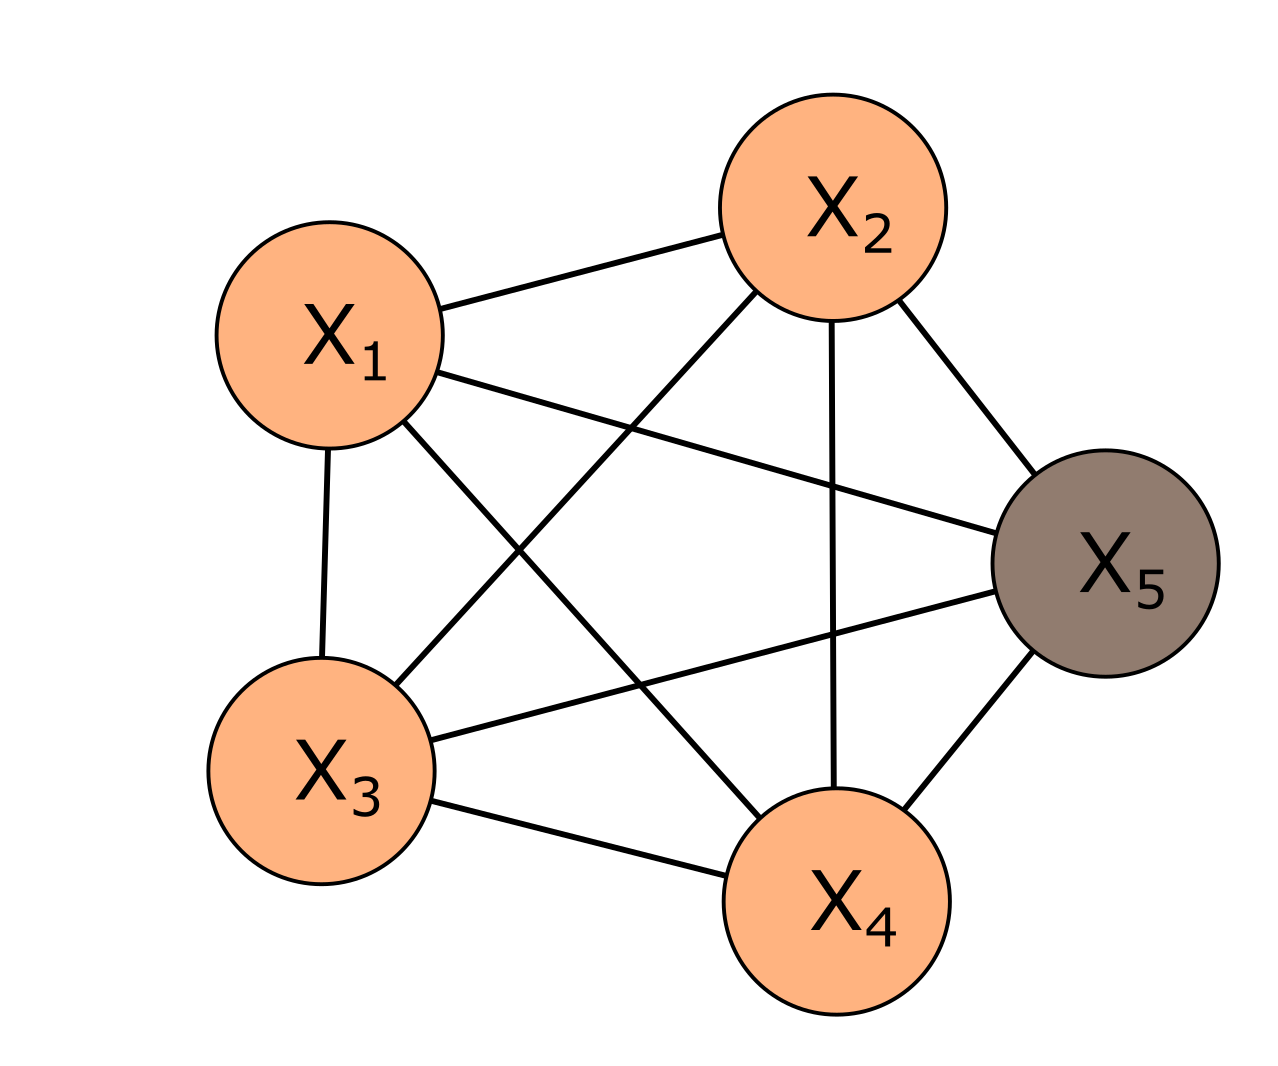
\includegraphics[scale=0.5]{images/bm_1.png}
    \caption{Diagrama de uma máquina de Boltzmann.\\
            \;}
  \end{figure}
\end{frame}

\begin{frame}{Arquitetura de BMs}%
  \begin{figure}[h]{}%
    \label{fig:bm-diagram}%
    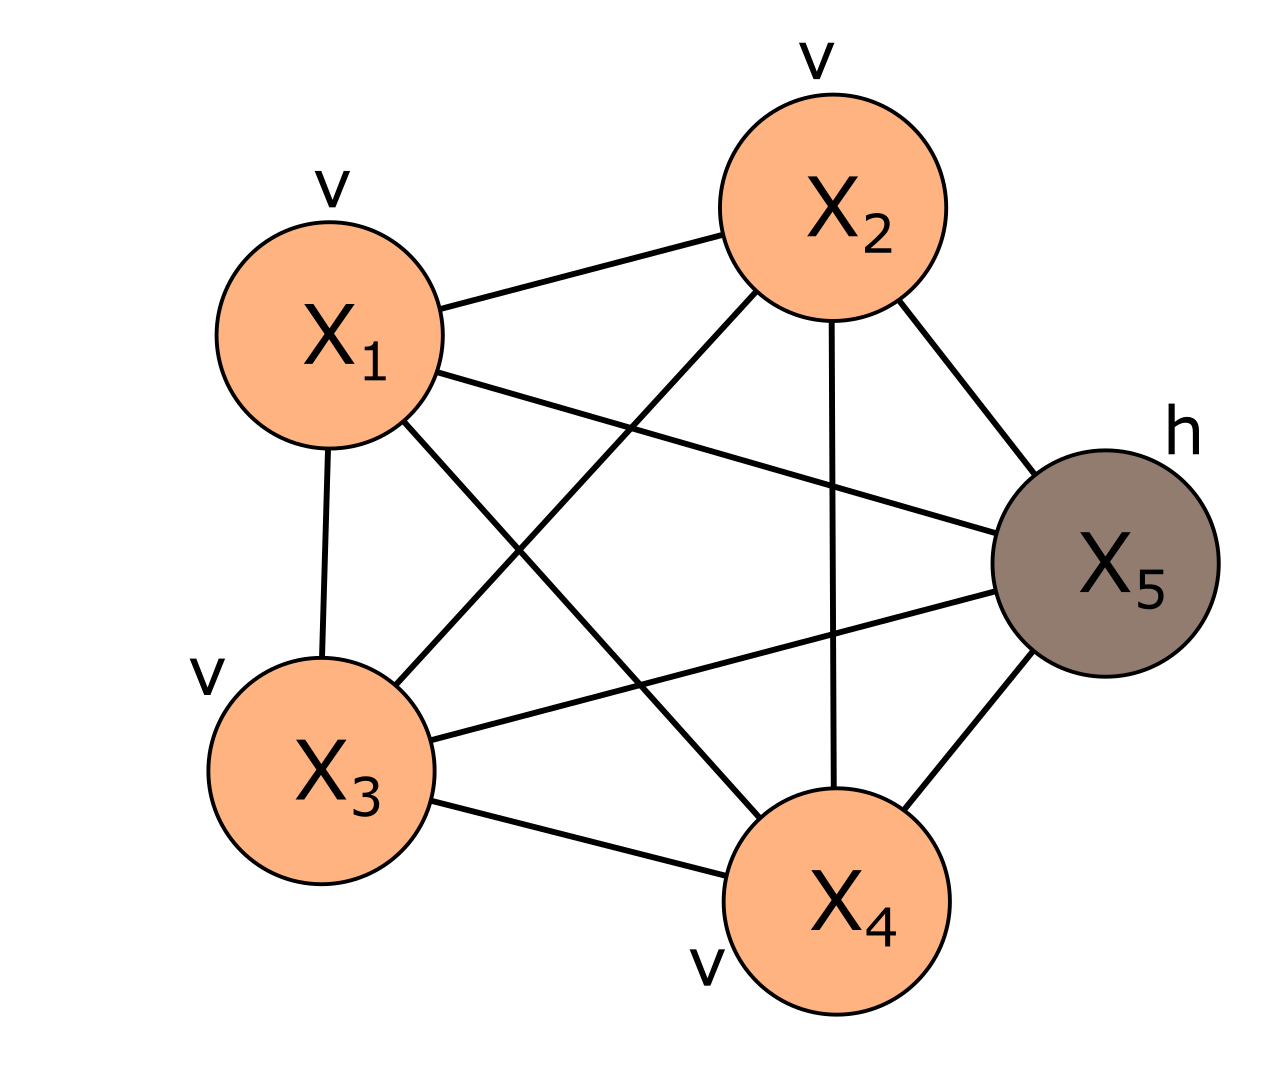
\includegraphics[scale=0.5]{images/bm_2.png}
    \caption{Diagrama de uma máquina de Boltzmann; unidades mais claras são as visíveis, e unidades mais escuras, as escondidas.}
  \end{figure}
\end{frame}

\subsection{Funcionalidade}%
\begin{frame}{}%
  \justiying%
  Na máquina de Boltzmann fazemos o ajuste das conexões $\omega_{ij}$ para termos um certo estado nas unidades visíveis com uma distribuição de probabilidade desejada.
\end{frame}


\begin{frame}{frame teste}
%  Suponhamos que queremos, que temos um problema onde queremos saber descrever a distribuição de probabilidade com que certos eventos acontecem.
%  
%  a partir de um conjunto de treinamento, determinar a distribuição de probabilidade de encontrar os estados mais estáveis da rede
\end{frame}
